\documentclass[11pt]{report}
\usepackage{geometry}
\geometry{letterpaper, margin=0.25in}
\usepackage{amsmath}
\usepackage{amssymb}
\usepackage{amsfonts}
\usepackage{dsfont}
\usepackage{epsfig}
\usepackage{times}
\usepackage{multicol}
%\usepackage{mcode}

\usepackage{bbm}

\usepackage{footnote}
\makesavenoteenv{tabular}

\usepackage{enumerate}
%\usepackage{enumitem}
\usepackage{pdfpages}
%\usepackage{hyperref}
\usepackage{calc}
\usepackage{verbatim}

\DeclareMathOperator{\Prob}{\mathbb{P}}
\DeclareMathOperator{\Exp}{\mathbb{E}}
\DeclareMathOperator{\Var}{\text{Var}}
\DeclareMathOperator*{\argmin}{\arg\min}
\DeclareMathOperator{\SSS}{\mathcal{S}}

\newcommand{\ind}{{\mathbbm{1}}}

\newcommand{\bs}{\boldsymbol}

\newcommand{\be}{\begin{enumerate}}
\newcommand{\ee}{\end{enumerate}}

\newcommand{\teq}{\triangleq}
\newcommand{\tr}{{\text{\tiny T}}}

\newcommand{\E}{\mathbb{E}}
\newcommand{\Ec}{\mathcal{E}}
\newcommand{\ep}{\varepsilon}

\newcommand{\abs}[1]{\left\vert #1 \right\vert} 
\newcommand{\ceil}[1]{\left\lceil #1 \right\rceil}
\parindent = 0cm
\parskip=5pt

\usepackage{tikz}
\usepackage{pgfplots}
\usepackage{tikz-cd}
\pgfplotsset{compat=1.18}
\usetikzlibrary{intersections, calc, decorations.markings}
\usepgfplotslibrary{polar}

\begin{document}
\begin{center}
    {\bf\large APMA 1740/2610 2025: Homework 2}
\end{center}
%\noindent{\bf\Large BE SURE TO CHANGE TO THE APPROPRIATE HW NUMBER}
\medskip


\begin{enumerate}[1.]

    \item {\bf Strange outcome, fair die.} Let $X_{1:n}$ be the outcomes of iid rolls of a fair six-sided die with faces labeled $\{1,\dotsc,6\}$.
          Define the empirical distribution $\widehat p \triangleq \bigl(\widehat p_1(X_{1:n}),\dotsc,\widehat p_6(X_{1:n})\bigr)$ by
          \[ \widehat p_x \triangleq \frac{1}{n}\sum_{i=1}^n \ind_{X_i=x} \]
          When $n$ is large the average outcome will typically be about 3.5 because of the LLN, i.e,
          \[ \bar X \triangleq \frac{1}{n}\sum_{i=1}^n X_i = \sum_{x=1}^6 x \widehat p_x \approx \sum_{x=1}^6 x \frac{1}{6} = 3.5 \]
          Suppose, however, that you observe the rare event
          \begin{equation} 3.0 < \bar X < 3.2 \label{e1} \end{equation}

          \begin{enumerate}[(a)]

              \item Use large deviations theory to guess the value of $\widehat p$,
                    i.e. guess the empirical distribution conditioned on observing a rare sample mean in the sense of equation \eqref{e1}.
                    Let's call your guess $p^*$.  Assume that $n$ is very large.  Your answer should be a table of 6 numbers.  Hint: (i) There are two constraints here
                    (defined by the two inequalities in (\ref{e1})), but only one can be active.  (ii) Once you decide on an active constraint, say $\Exp[{\mathcal E}(X)]=\theta$, you have to determine the parameter $\lambda$ in the Gibbs representation of $p^*$.  Do this by gradient descent on the log-partition function (actually, on $\log Z_\lambda - \lambda\theta$) as described in class.  Check your $\lambda$ to make sure that the constraints are (approximately) satisfied.

                    \color{blue}
                    Let $B = \{q: \E_q[X] \in (3.0, 3.2)\}$

                    By the LDP, we are interested in
                    \[p^* = \argmin_{q \in B} D(q \parallel \hat p)\]
                    subject to the constraints
                    \begin{itemize}
                        \item $\E[\Ec(X)] < 3.2$
                        \item $\E[\Ec(X)] > 3.0$
                    \end{itemize}

                    Let us begin with the active constraint $\E[\Ec(X)] = 3.2$ since $\bar X = 3.5 > 3.2$ and Sanov implies the $p^*$ will occur on the boundary.

                    From previous work, we know the solution to the minimization problem is given by
                    \[p_x^* = \frac{1}{Z_{\lambda}} \hat p_x e^{\lambda x}\]
                    where $Z_{\lambda} = \sum_{x=1}^6 \hat p_x e^{\lambda x}$.

                    We need now to solve for $\lambda$. Luckily, we know that
                    \[\frac{\partial}{\partial \lambda} = \log Z_{\lambda} - 3.2\lambda = \E_{\lambda}[X] - 3.2 = -3.2 + \sum_{x=1}^{6} \frac{x \cdot p_x^{\lambda x}}{Z_{\lambda}}\]

                    is convex in $\lambda$ and minimized when $\E_{\lambda}[\Ec(X)] = 3.2$, i.e. at exactly the $\lambda$ we need to find.

                    Let $\lambda^{(0)} = \frac{1}{6}$ and $\ep = 10^{-6}$. We will use gradient descent to find the optimal $\lambda$ by:
                    \[\lambda^{(t + 1)} = \lambda^{(t)} - (\E_{\lambda}[X] - \theta)\]
                    until $\abs{\lambda^{(t+1)} - \lambda^{(t)}} < \ep$.

                    Running the algorithm, we find
                    \[\lambda \approx -0.1031\]
                    and
                    \begin{align*}
                        p^*_1 & \approx 0.217 \\
                        p^*_2 & \approx 0.192 \\
                        p^*_3 & \approx 0.173 \\
                        p^*_4 & \approx 0.156 \\
                        p^*_5 & \approx 0.140 \\
                        p^*_6 & \approx 0.127
                    \end{align*}

                    \color{black}


              \item {\color{blue} (Do not submit)} Perform a series of Monte Carlo computer experiments: For each of \\$n=50,100,150,\dotsc,400$, repeatedly sample $n$ rolls of a fair die.\footnote{An easy way to do this in Matlab is with the command {\tt randi(6,n,1)}.}  For each sample of size $n$, check for the rare event from equation \eqref{e1}.  Accumulate $m=100$ examples of this event for each value of $n$.  Let $M$ be the number of samples needed to see $m$ events,\footnote{You can get a rough idea of how big $M$ will need to be from the CLT, which says that $\bar X$ is approximately Normal with mean 3.5 and variance $\sigma^2/n$, where $\sigma^2$ is the variance of a single $X_i$.} so that $m/M$ is an estimate of the probability of the rare event.  Let $\widehat p^{(1)},\dotsc,\widehat p^{(m)}$ be the observed empirical distributions for each of the $m$ rare events and let $\Delta_1,\dotsc,\Delta_m$ be the corresponding distances from the empirical distributions to your prediction $p^*$ above, where the distance is defined as
                        \[
                            \Delta_k \triangleq \max_{1\leq x \leq 6} \bigl|p_x^*-\widehat p_x^{(k)}\bigr| \qquad k=1,\ldots,m
                        \]
                        Let $\bar\Delta$ and $S_{\Delta}$ be the empirical mean and standard deviation of the $\Delta_k$'s, respectively.

                        Plot $m/M$, $\frac{1}{n}\log(m/M)$, $\bar\Delta$, and $S_{\Delta}$ versus $n$.  Interpret the four plots.

                    \color{blue}
                    \begin{center}
                        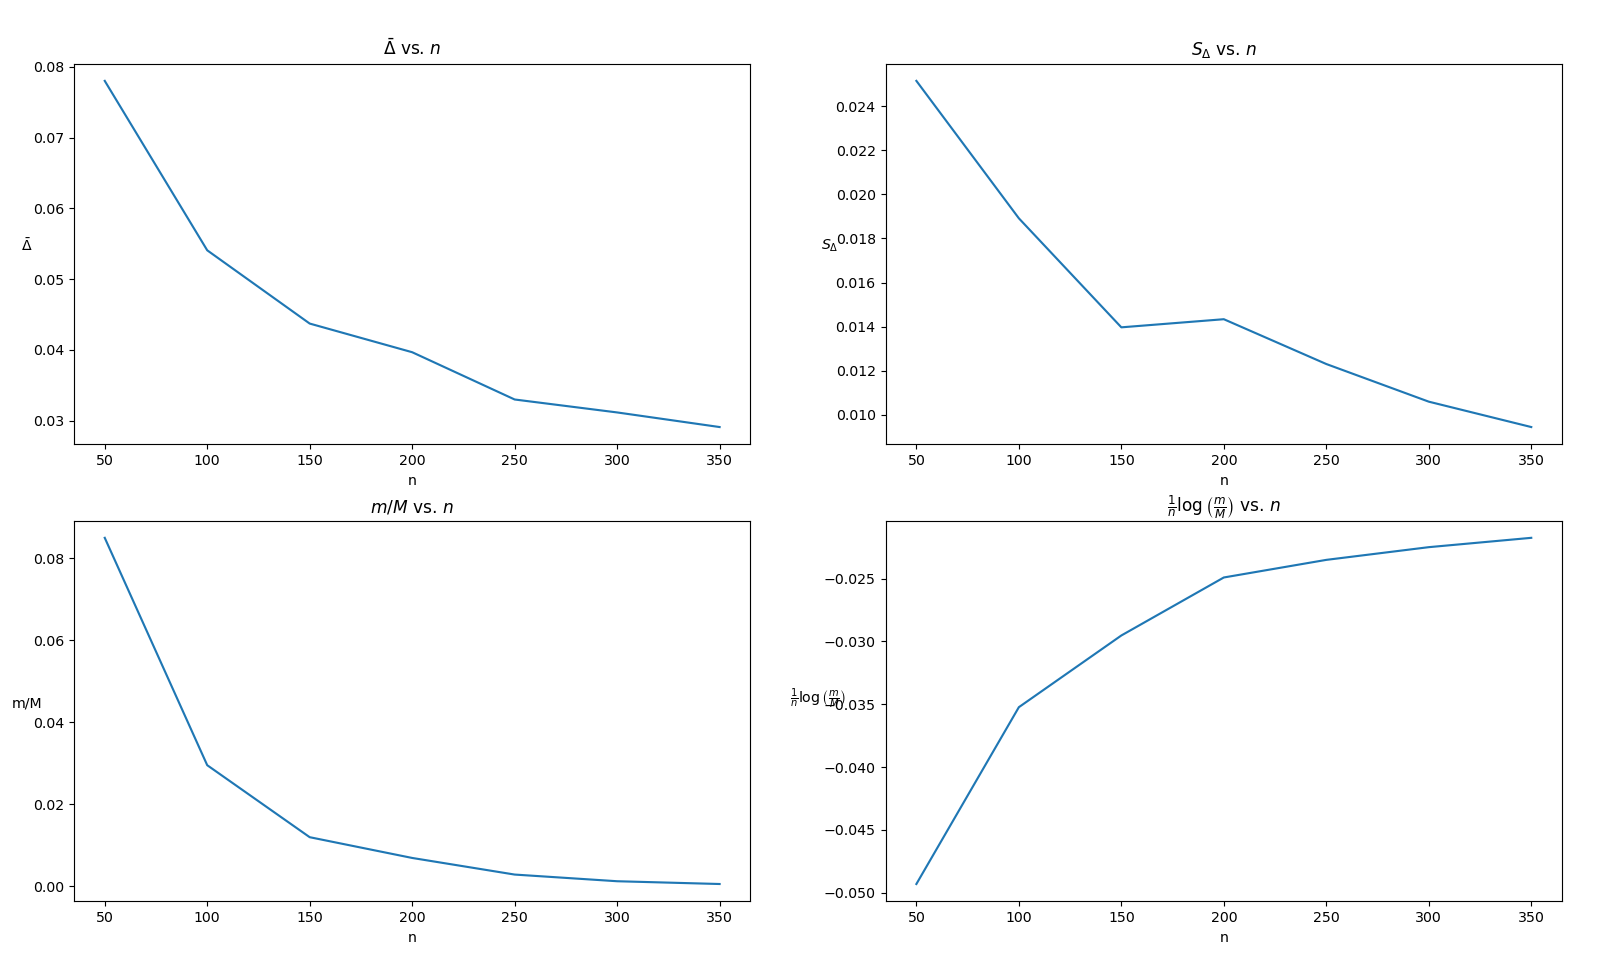
\includegraphics[width=0.9\textwidth]{1b.png}
                    \end{center}
                    \color{black}

              \item For each of the four plots, as $n\to\infty$, what is the limiting value of each quantity?  Why?

                    \color{blue}
                    All four plots go to $0$ as $n\to \infty$. As $n$ increases, LLN says we should see the rare event less and less frequently, so $m/M$ should go to $0$. The LLN also says that the empirical distribution should converge to the true distribution, so $\bar \Delta$ and $S_{\Delta}$ should go to $0$ as well. We expect $\log(m/M) \to -\infty$ but $1/n \to 0$ more quickly and we take the convention $0\log 0 = 0$.
                    \color{black}

          \end{enumerate}

          \pagebreak

    \item  {\color{blue} (Do not submit)} {\bf Strange outcome, weighted die.} Repeat problem 1 using an {\em un}-fair die with \\ $h=(h_1,\dotsc,h_6)=(.1,.1,.2,.1,.2,.3)$ and with the rare event defined by {\em both}
          %\begin{subequations} \label{e2}
          \begin{equation*}
              3.6 < \bar X < 3.8  %\label{e2a} 
          \end{equation*}
          and
          \begin{equation*}
              U \triangleq \frac{1}{n}\sum_{i=1}^n X_i^2 < 17 %\label{e2b} 
          \end{equation*}
          %\end{subequations}
          Note that both of these are unusual for large $n$, since we expect $\bar X \approx 4.1$ and $U\approx 19.7$ from the LLN.  For part (a) you will need to determine which constraints are active.  Try each individually and see if the other is satisfied.  If neither works individually, you will need to use both simultaneously.  For part (b) only use $n=50,100,150,\dotsc,300$.\footnote{An easy way to simulate this particular unfair die in Matlab is to first define the table {\tt lookup = [1 2 3 3 4 5 5 6 6 6]} and then get $n$ rolls with {\tt lookup(randi(10,n,1))}.}

          \pagebreak

    \item {\bf Exponential families.}
          The exponential families first came up as solutions to the maximum entropy problem under a set of $c$ constraints
          \begin{equation}
              \label{eqn:C1}
              \mathds{E}_p[{\cal E}_k(X)] = \theta_k \qquad k=1,2,\ldots, c
          \end{equation}
          We called these constraints {\em linear}, since they are linear in the components of $p^*$, as can be seen by writing out, explicitly, the expectation in (\ref{eqn:C1}):
          \[
              \sum_{x=1}^s p^*(x){\cal E}_k(x) = \theta_k \qquad k=1,2,\ldots, c
          \]
          Solving the optimization problem led us to exponential families of the form
          \[
              p^*(x) = \frac{1}{Z_{\lambda_1,\ldots,\lambda_c}}e^{\sum_{k=1}^c \lambda_k {\cal E}_k(x)}\qquad \forall x\in \{1, \ldots,s\}
          \]
          The more general LDP problem (minimize $D(q||p)$ given a pmf $p$ on $\{1,\ldots,s\}$), under these very same constraints, led us instead to a more general collection of exponential families, namely all distributions on $\{1, \ldots,s\}$ of the form
          \[
              p^*(x) = \frac{p(x)}{Z_{\lambda_1,\ldots,\lambda_c}}e^{\sum_{k=1}^c \lambda_k {\cal E}_k(x)}\qquad \forall x\in \{1, \ldots,s\}
          \]

          These derivations were in the context of discrete ($X \in \{1, \ldots,s\}$) and univariate ($X \in \mathds{R}^1$) random variables. But the approach is more general, in two important ways: (i) we could just as well have started with continuous random variables that had density functions instead of probability mass functions (see, for example, problem 5 on this HW), and (ii) we could also have started with multivariate random variables, also known as random vectors, in $d$ dimensions ($X\in\mathds{R}^d$).

          Let $X$ be a continuous or discrete random variable with a pdf or pmf $f(x) = f(x;\vec{\lambda})$, where $\vec{\lambda} = \{\lambda_1,\ldots,\lambda_c\}$ is a collection of parameters that define a family of distributions. This is an ``exponential family" with ``canonical'' or ``natural'' parametrization if $f$ can be written in the form
          \begin{equation}
              \label{eqn:exp_family}
              f(x;\vec{\lambda}) = \frac{1}{Z(\vec{\lambda})}p(x)e^{\vec{\lambda}\cdot\vec{\cal E}(x)}
          \end{equation}
          where $p(x)$ is any function that is non-negative on the range of $X$, and
          $\vec{\cal E}(x) = ({\cal E}_1(x),\ldots,={\cal E}_c(x))$ are the ``sufficient statistics''.\footnote{In statistics, $T_k(x)$, $k=1,\ldots,c$ is traditional. We used ${\mathcal E}_k$, since these arose as energies in the Gibbs thought experiment.}
          (As we shall see in class, there is indeed something canonical about the canonical parametrization. Namely, that the normalizing constant, i.e. the ``partition function" $Z(\vec{\lambda})$, becomes
          the key to computing the values of the parameters, whether we are given samples and want to do maximum-likelihood estimation or we want to compute an LDP distribution from the $\theta$ parameters.)
          Nothing about this representation is unique---the same family can be written with different  parameters and different sufficient statistics, and $p$ and $Z$ can be multiplied by a common arbitrary constant,
          since this will not change the ratio.
          As for the generalization to multivariate $X$, instead of mapping $\mathds{R}^1$ to $\mathds{R}^1$, $f$, $p$, and the sufficient statistics ${\cal E}_1,\ldots,{\cal E}_c$ map
          $\mathds{R}^n$ to $\mathds{R}^1$.

          The problem is to determine which of the following standard statistical families is an exponential family. For any that are, identify the sufficient statistics.
          \begin{enumerate}[(a)]
              \item Binomial$(100,p)$ with parameter $p\in[0,1]$. (Hint: start by writing $f$ as
                    \[f(x) = {100\choose x}p^x(1-p)^{100-x}\ind_{x\in\{0,1,\ldots,100\}}\] and note that this one-parameter family will have only one sufficient statistic, and the associated $\lambda$ will be a function of $p$: $\lambda = \lambda(p)$.)

                    \color{blue}
                    \begin{align*}
                        f(x) & = {100\choose x}p^x(1-p)^{100-x}\ind_{x\in\{0,1,\ldots,100\}}                             \\
                             & = {100\choose x} \left(\frac{p}{1-p}\right)^x (1 - p)^{100} \ind_{x\in\{0,1,\ldots,100\}} \\
                             & = {100 \choose x} e^{x\log \frac{p}{1 - p} + 100\log(1- p)}\ind_{x\in\{0,1,\ldots,100\}}
                    \end{align*}

                    Let $h(x) = {100 \choose x} \ind_{x \in \{0, 1, \dots, 100\}}$, $\Ec(x) = x$, and $\lambda(p) = \log \frac{p}{1 - p}$. Then
                    \[f(x) = \frac{1}{Z(\lambda)} p(x) e^{\lambda \Ec(x)}\]
                    where
                    \[\frac{1}{Z(\lambda)} = e^{100\log (1 - p)} = e^{100 \log \frac{1}{1 + e^{\lambda}}} = (1 + e^{\lambda})^{-100} \implies Z(\lambda) = (1 + e^{\lambda})^{100}\]
                    \color{black}

              \item Binomial$(n,p)$ for parameter $(n,p)$

                    \color{blue}
                    Analogously,
                    \[f(x) = {n\choose x}p^x(1-p)^{n-x}\ind_{x\in\{0,1,\ldots,n\}}\]
                    so with
                    \begin{align*}
                        h(x)       & = {n\choose x} \ind_{x\in\{0,1,\ldots,n\}} \\
                        \Ec(x)     & = x                                        \\
                        \lambda(p) & = \log \frac{p}{1 - p}                     \\
                        Z(\lambda) & = (1 + e^{\lambda})^n
                    \end{align*}
                    we have
                    \[f(x) = \frac{1}{Z(\lambda)} p(x) e^{\lambda \Ec(x)}\]
                    \color{black}

              \item  {\color{blue} (Do not submit)} Normal$(\mu,\sigma^2)$ for parameter $(\mu,\sigma^2)$
              \item Uniform$(0,m)$ for parameter $m$

                    \color{blue}
                    \[f(x) = \frac{1}{m}\ind_{x\in[0,m]}\]
                    but this has no parameter, so it is not an exponential family.
                    \color{black}

              \item  {\color{blue} (Do not submit)} Gamma$(\alpha,\beta)$ for parameter $(\alpha,\beta)$ (i.e. $\displaystyle
                        f(x;\alpha,\beta) = \frac{\beta^\alpha}{\Gamma(\alpha)}\ind_{x>0}x^{\alpha-1}e^{-\beta x}$)
          \end{enumerate}

          \pagebreak

    \item {\bf Samples from an exponential family.} Let $X_{1:n}$ be iid from an exponential family with sufficient statistics $\vec{\cal E}={\cal E}_{1:c}$ over $\mathbb{R}$. Show that the joint distribution of $X_{1:n}$ is an exponential family over $\mathbb{R}^n$ and identify the sufficient statistics.

          \color{blue}
          Since $X_{1:n}$ are iid, the joint distribution is
          \begin{align*}
              f(x_1, \dots, x_n; \vec \lambda) & = \prod_{k=1}^n f(x_k; \vec \lambda)                                                                         \\
                                               & = \prod_{k=1}^n \frac{1}{Z(\vec \lambda)} p(x_k) e^{\vec \lambda \cdot \Ec(x_k)}                             \\
                                               & = \frac{1}{Z(\vec \lambda)^n} \left(\prod_{k=1}^n p(x_k)\right) e^{\vec \lambda \cdot \sum_{k=1}^n \Ec(x_k)} \\
          \end{align*}

          If we define $\tilde Z(\vec \lambda) = Z(\vec \lambda)^n$, $\tilde p(x_1, \dots, x_n) = \prod_{k=1}^n p(x_k)$, and $\tilde \Ec(x_1, \dots, x_n) = \sum_{k=1}^n \Ec(x_k)$, then we have
          \[f(\vec x; \vec \lambda) = \frac{1}{\tilde Z(\vec \lambda)} \tilde h(\vec x) e^{\vec \lambda \cdot \tilde \Ec(\vec x)} \]
          where each $\tilde \Ec_{1:c} = \sum_{k=1}^n \Ec_{1:c}(x_k) = n \bar{\Ec}$.
          \color{black}

          \pagebreak

    \item {\bf The partition function has a few more tricks up its sleeve.}
          A common theme in statistical mechanics is the deep relationship between the properties of a physical system and the partition function of its equilibrium distribution. A similar theme emerges in
          statistics, as illustrated by our derivation, in the lectures, of a collection of properties relating
          derivatives of the partition function to the computation of parameters in exponential families. In this problem we will exploit this connection further, in order to get closed form solutions to some expectations that would be otherwise very difficult to compute.

          Let $X$ be a continuous random variable with pdf $f(x) = f(x;\vec{\lambda})$, where $\lambda = \{\lambda_1,\ldots,\lambda_c\}$ is a collection of parameters that define a family of distributions. This is an ``exponential family with ``canonical'' or ``natural'' parametrization if $f$ can be written in the form
          \begin{equation}
              \label{eqn:exp_family}
              f(x;\lambda) = \frac{1}{Z(\lambda)}p(x)e^{\vec{\lambda}\cdot
                      T(x)}
          \end{equation}
          where $p(x)$ is any function that is everywhere non-negative and
          $T(x) = (T_1(x),\ldots,T_c(x))$ are the ``sufficient statistics''.\footnote{In statistics, $T$ (instead of ${\mathcal E}$) is traditional.}
          This problem is about the particular family of pdfs defined by
          \[
              f(x;\beta) = \frac{\ind\{x > 0\}}{\sqrt{2\pi x^3}}\exp\left(-\frac{(x-\beta)^2}{2x\beta^2}\right)
          \]
          for $x\in\mathbb{R}$ and parameter $\beta > 0$. The purpose of this problem is to use properties of exponential families to compute the mean and variance of $X$ in terms of $\beta$.

          But before jumping into it, let's pause to consider the direct approach, which means finding closed form expression for two integrals:
          \[
              \mu \doteq \Exp[X] = \int_0^\infty \frac{x}{\sqrt{2\pi x^3}}\exp\left(-\frac{(x-\beta)^2}{2x\beta^2}\right) dx
              \quad
              \sigma^2 \doteq \Var[X] = \int_0^\infty \frac{(x-\mu)^2}{\sqrt{2\pi x^3}}\exp\left(-\frac{(x-\beta)^2}{2x\beta^2}\right) dx
          \]
          Not an easy task. So let's come at it from a different direction:


          \begin{enumerate}[(a)]
              \item Show that $f$ can be expressed as an exponential family of the form given in equation (\ref{eqn:exp_family}), where
                    $\lambda = \lambda(\beta)$ is a scalar function of $\beta$.
                    Explicitly identify the function $\lambda(\beta)$, as well as $p(x)$,  $T(x)$, and $Z(\lambda)$. (For the latter, be sure to write $Z$ in terms of $\lambda$ and not $\beta$.)

                    \color{blue}
                    \begin{align*}
                        f(x; b) & = \frac{\ind\{x> 0\}}{\sqrt{2\pi x^3}} \exp\left(-\frac{(x- \beta)^2}{2x\beta^2}\right)                      \\
                                & = \frac{\ind\{x> 0\}}{\sqrt{2\pi x^3}} \exp\left(-\frac{x^2 - 2x\beta + \beta^2}{2x\beta^2}\right)           \\
                                & = \frac{\ind\{x> 0\}}{\sqrt{2\pi x^3}} \exp\left(-\frac{x}{2\beta^2} + \frac{1}{\beta} - \frac{1}{2x}\right) \\
                                & = \frac{\ind\{x> 0\}}{\sqrt{2\pi x^3}} e^{1/\beta} e^{-1/2x} e^{-x/2\beta^2}
                    \end{align*}

                    Hence with
                    \begin{align*}
                        p(x)           & = \frac{\ind\{x> 0\}}{\sqrt{2\pi x^3}}e^{-\frac{1}{2x}} \\
                        T(x)           & = -x                                                    \\
                        \lambda(\beta) & = \frac{1}{2\beta^2}                                    \\
                        Z(\lambda)     & = e^{1/\beta} = e^{\sqrt{-2\lambda}}
                    \end{align*}
                    we see that $f$ is an exponential family.
                    \color{black}

              \item Use the properties of (natural) exponential families that we proved in class to compute the mean and variance of $T(X)$ in terms of $\lambda$. For full credit, you must use properties of exponential families. In other words, you should be solving this problem with differentiation, not integration.

                    \color{blue}
                    In class, we showed that
                    \[\frac{\partial}{\partial \lambda} \log Z_{\lambda} = \E_{\lambda}[T_k(X)]\]

                    Hence,
                    \[\E_{\lambda}[T(X)] = \frac{\partial }{\partial \lambda} \log Z_{\lambda} = \frac{\partial}{\partial \lambda} \sqrt{2\lambda} = -\frac{1}{\sqrt{2\lambda}}\]

                    Further,
                    \[\frac{\partial^2}{\partial \lambda^2} \log Z_{\lambda}= \Var_{\lambda}(T(X))\]
                    so
                    \[\Var_{\lambda}[T(X)] = \frac{\partial^2}{\partial \lambda^2} \log Z_{\lambda}= -\frac{\partial}{\partial \lambda_1} \frac{1}{\sqrt{2\lambda}} = -(2\lambda)^{-3/2}\]
                    \color{black}

              \item Finally, use the function $\lambda(\beta)$ derived in (a) to express the mean and variance of $X$ in terms of $\beta$.

                    \color{blue}
                    We have $\lambda(\beta) = \frac{1}{2\beta^2}$, so
                    \begin{align*}
                        \E[X]   & = -\E[T(X)] = -\frac{1}{\sqrt{2\lambda}} = -\frac{1}{\sqrt{\frac{1}{\beta^2}}} = -\frac{1}{\frac{1}{\beta}} = \boxed{-\beta} \\
                        \Var[X] & = \Var[T(X)] = \left(-2\cdot \frac{1}{2\beta^2}\right)^{-3/2} = \boxed{-\beta^3}
                    \end{align*}
                    \color{black}

          \end{enumerate}
          This is almost magical. We sidestepped two daunting integrations
          by simply identifying $Z$ and then taking derivatives. But it wasn't quite a ``free lunch''---after all,  we were given the fact that $f$ is normalized, which is not so obvious. In any case, you can perhaps begin to see why a closed-form expression for the partition function is so highly valued when modeling physical systems with Gibbs and related distributions.




          %%%%%%%%%%%%%%%%%%%%%%%%%%%%%%%%%%%%%%%%%%%%%



          \pagebreak
    \item {\bf Prefix codes and uniquely decodable codes.}
          Recall that a binary code $C:\{1,\ldots,s\}\to\{0,1\}^*$ is a {\bf prefix code} (also known as ``instantaneous code'') if $C(x)$ is not the prefix of any other code word $C(y)$ (e.g. $001$ {\em is a prefix} of $0010$).
          On the other hand, $C$ is {\bf uniquely decodable}
          if any finite string of codewords has a unique decoding. In other words, if $C(x_1)\cdots C(x_i) = C(y_1)\cdots C(y_j)$ then
          $i=j$ and $x_k=y_k$ for each $k=1:i.$\footnote{Here, $x_k \in\{1,\ldots,s\},\ k=1:i$, are $i$ source symbols and $C(x_1)\cdots C(x_i)$ is the concatenation of the
              corresponding codes; the right-hand side is interpreted analogously.}

          Clearly, prefix codes are uniquely decodable (just read off the source symbols left-to-right), but uniquely decodable codes are not necessarily prefix codes. A theorem (proved in problem \ref{HW:Uniquely}) shows that for every uniquely decodable code, $C$, there is a prefix code $\tilde{C}$ with codewords of the same length, i.e. $|\tilde{C}(x)|=|C(x)|$ for all $x$.

          Consider the following three codes for the source $\{1,\ldots,4\}$:

          \begin{tabular}{c|lll}
              $x$ & $C_1(x)$ & $C_2(x)$ & $C_3(x)$ \\ \hline
              $1$ & $00$     & $0$      & $0$      \\
              $2$ & $01$     & $1$      & $01$     \\
              $3$ & $10$     & $01$     & $011$    \\
              $4$ & $11$     & $11$     & $111$
          \end{tabular}

          \begin{enumerate}
              \item For each of the three codes, list all possible decodings of $001111$.

                    \color{blue}
                    \qquad \begin{tabular}{ccc}
                        $C_1$ & $C_2$  & $C_3$ \\\hline
                        144   & 112222 & 124   \\
                              & 11224          \\
                              & 11242          \\
                              & 11422          \\
                              & 1144           \\
                              & 13222          \\
                              & 1324           \\
                              & 1342           \\\hline
                    \end{tabular}
                    \color{black}

              \item Which of these codes is uniquely decodable? Why?

                    \color{blue}
                    Only $C_1$ and $C_3$ are uniquely decodable since $C_1$ is prefix and $\sum 2^{-\abs{C_3(x)}} = 1 \leq 1$ so $C_3$ is uniquely decodable by Kraft-McMillan.
                    \color{black}

              \item One of these codes is uniquely decodable but not prefix. Find a prefix code with the same code lengths.

                    \color{blue}
                    \qquad \begin{tabular}{c|l}
                        $x$ & $\tilde{C}_3(x)$ \\ \hline
                        $1$ & $0$              \\
                        $2$ & $10$             \\
                        $3$ & $110$            \\
                        $4$ & $111$
                    \end{tabular}

                    is prefix and has the same code lengths as $C_3$.
                    \color{black}

              \item If $p=p_{1:4}=(.7,.1,.1,.1)$ (a probability on the source), then
                    $\mathbb{E}_p|C(X)| \doteq \sum_{x=1:4} |C(x)|p_x$ is the average number of bits per symbol. Compute $\mathbb{E}_p|C(X)|$ for each of these three codes, and compare these averages to the entropy $H(p)$ (remember to use $\log_2$). Comment on which code might be the most useful.

                    \color{blue}
                    \begin{align*}
                        \E_p\abs{C_1(X)} & = 0.7\cdot \abs{C_1(1)} + 0.1\cdot \abs{C_1(2)} + 0.1\cdot \abs{C_1(3)} + 0.1\cdot \abs{C_1(4)} \\
                                         & = 0.7\cdot 2 + 0.1\cdot 2 + 0.1\cdot 2 + 0.1\cdot 2 = \boxed{2}                                 \\
                        \E_p\abs{C_2(X)} & = 0.7\cdot \abs{C_2(1)} + 0.1\cdot \abs{C_2(2)} + 0.1\cdot \abs{C_2(3)} + 0.1\cdot \abs{C_2(4)} \\
                                         & = 0.7\cdot 1 + 0.1\cdot 1 + 0.1\cdot 2 + 0.1\cdot 2 = \boxed{1.2}                               \\
                        \E_p\abs{C_3(X)} & = 0.7\cdot \abs{C_3(1)} + 0.1\cdot \abs{C_3(2)} + 0.1\cdot \abs{C_3(3)} + 0.1\cdot \abs{C_3(4)} \\
                                         & = 0.7 \cdot 1 + 0.1\cdot 2 + 0.1\cdot 3 + 0.1\cdot 3 = \boxed{1.5}
                    \end{align*}
                    but
                    \[H(p) = -\sum_{x=1}^4 p_x \log_2 p_x = - (0.7)(\log_2 0.7) - (3)(0.1)(\log_2 0.1) \approx 1.3568\]

                    By a Theorem from class, the optimal code $C^*$ satisfies
                    \[H(p) \leq \E_p \abs{C^*} \leq H(p) + 1\]
                    so we know an optimal code must satisfy
                    \[1.3568 \leq \E_p \abs{C^*} \leq 2.3568\]

                    Hence both $C_1$ and $C_3$ are candidates and are uniquely decodable. Since $C_3$ has the shorter expected code length, however, it is likely to be more useful.
                    \color{black}

              \item Repeat part (d) for $p=(.1,.1,.1,.7)$.

                    \color{blue}
                    \begin{align*}
                        \E_p\abs{C_1(X)} & = 0.1\cdot 2 + 0.1\cdot 2 + 0.1\cdot 2 + 0.7\cdot 2 = \boxed{2}   \\
                        \E_p\abs{C_2(X)} & = 0.1\cdot 1 + 0.1\cdot 1 + 0.1\cdot 2 + 0.7\cdot 2 = \boxed{1.8} \\
                        \E_p\abs{C_3(X)} & = 0.1\cdot 1 + 0.1\cdot 2 + 0.1\cdot 3 + 0.7\cdot 3 = \boxed{2.7}
                    \end{align*}
                    and
                    \[H(p) = -(3)(0.1)(\log_2 0.1) - (0.7)(\log_2 0.7) \approx 1.3568 \]

                    In this case, $C_3$ is no longer in the optimal range and $C_2$ is not uniquely decodable. Hence $C_1$ is the best code.
                    \color{black}


          \end{enumerate}



          %%%%%%%%%%%%%%%%%%%%%%%%%%%%%%%%%%%%%%%%%%%%%



          \pagebreak

    \item {\bf Block coding.} Let $X_1,X_2,\dotsc$ be iid with pmf $p=p_{1:2}=(0.3,0.7)$. Find a binary and uniquely decodable code $C$ on the source $\{1,2\}$ that has expected code length per source symbol within $0.025$ bits of the smallest possible value. (You might need to encode blocks.)

          \color{blue}
          We know that for $C_n^* = \argmin_{C_n} \E\abs{C(X_{1:n})}$,
          \[H(p) \leq \frac{1}{n}\E\abs{C^*_n(X_{1:n})} \leq H(p) + \frac{1}{n}\]

          Since we want to be within $0.025$ bits of the optimal code, we need $n = \frac{1}{0.025} = 40$.

          We can calculate
          \[H(p) = -0.3\log_2 0.3 - 0.7\log_2 0.7 \approx 0.881\]

          So we need
          \[0.881 \leq \frac{1}{40} \E\abs{C(X_{1:n})} \leq 0.906\]

          We also know that for each symbol, we will need roughly $\log \frac{1}{0.3} \approx 1.7$ and $\log \frac{1}{0.7} \approx 0.5$ bits so it is reasonable to use blocks of length 2.

          Now,

          \qquad \begin{tabular}{cc}
              $x$ & $p(x)$ \\ \hline
              11  & 0.09   \\
              12  & 0.21   \\
              21  & 0.21   \\
              22  & 0.49
          \end{tabular}

          We want the highest probability symbols to have the shortest code lengths, so consider the code:

          \qquad \begin{tabular}{cl}
              $x$ & $C(x)$ \\ \hline
              11  & 111    \\
              12  & 110    \\
              21  & 10     \\
              22  & 0
          \end{tabular}

          which is prefix and has
          \[\E\abs{C(x)} = 0.09(3) + 0.21(3) + 0.21(2) + 0.49(1) = 1.81 \implies 0.905 \text{ bits/symbol}\]
          which is within the desired range.


          \color{black}


          %%%%%%%%%%%%%%%%%%%%%%%%%%%%%%%%%%%%%%%%%%%%%
          \pagebreak





    \item {\bf Shannon codes.} Let $X_{1:n}$ be iid Bernoulli$(p)$, with $p=0.2$.  For each positive integer $n$, each $q\in(0,1)$ and each $x_{1:n}\in\{0,1\}^n$, define
          \[ f_{n,q}(x_{1:n}) \teq \prod_{i=1}^n q^{x_i}(1-q)^{1-x_i} \]
          which is the probability mass function of $n$ iid Bernoulli$(q)$ random variables.

          \begin{enumerate}
              \item Use the Kraft-McMillan theorem to show that, for each positive integer $n$ and each $q\in(0,1)$, there exists a (variable length, binary) prefix code, say $C_{n,q}$, over $\{0,1\}^n$ (a source with $s=2^n$ symbols) with
                    \[ |C_{n,q}(x_{1:n})| = \lceil-\log_2 f_{n,q}(x_{1:n})\rceil \]
                    for all $x_{1:n}\in\{0,1\}^n$, where $\lceil a \rceil$ is the ceiling function, i.e., the smallest integer greater than or equal to $a$.
                    (This ``Shannon code'' was the key construction in our proof of Corollary 1 to the Kraft-McMillan Inequality.)

                    \color{blue}
                    By the Kraft-McMillan Inequality, for any code lengths $\ell_1, \dots, \ell_{2^n}$ with
                    \[\sum_{x=1}^{2^n} 2^{-\ell_x} \leq 1\]
                    there exists a prefix code with $\abs{C(x)} = \ell_x$.

                    In particular, this means that for any $n$ and $q$, it suffices to show that
                    \[\sum_{x=1}^{2^n} 2^{-\ell_x} = \sum_{x=1}^{2^n} 2^{-\ceil{-\log_2 f_{n, q}(x_{1:n})}} \leq 1\]

                    And in fact,
                    \color{blue}
                    \begin{align*}
                        \sum_{x=1}^{2^n} 2^{-\ceil{-\log_2 f_{n, q}(x_{1:n})}} & \leq \sum_{x=1}^{2^n} 2^{\log_2 f_{n, q}(x_{1:n} + 1)} \\
                                                                               & = \sum_{x=1}^{2^n} f_{n, q}(x_{1:n})                   \\
                                                                               & = \sum_{x=1}^{2^n} \prod_{i=1}^n q^{x_i}(1-q)^{1- x_i} \\
                                                                               & = (q + [1 - q])^n                                      \\
                                                                               & = 1^n = 1
                    \end{align*}
                    \color{black}


              \item {\color{blue} (Do not submit)} For all $(q,n)$ combinations of $q=.01,.1,.2,.5,.8$ and $n=1,2,3,4,5,10,20,100,500$, approximate $\frac{1}{n}\Exp|C_{n,q}(X_{1:n})|$ by generating $10^5$ independent realizations of $X_{1:n}$ and averaging the corresponding code lengths for each realization (and then divide by $n$).\footnote{One way to generate $X_{1:n}$ in Matlab is {\tt (rand(1,n)<p)}. Also, {\tt ceil} is the ceiling function in Matlab.}  As $n$ varies, this gives a graph for each of the five values of $q$.  Plot these 5 graphs on the same plot.\footnote{The matlab command {\tt hold on} will let you put multiple graphs on the same plot. Use {\tt hold off} to stop this behavior and revert to the default where each plotting command clears the current plot.}

              \item {\color{blue} (Do not submit)}   For each of the five values of $q$, compute the limiting value as $n\to\infty$, i.e.,
                    \[ \lim_{n\to\infty}\frac{1}{n}\Exp|C_{n,q}(X_{1:n})| \]
              \item {\color{blue} (Do not submit)}  Interpret the graphs.  Which code is best?  Is it possible to do much better than this code?  Why or why not?
          \end{enumerate}


          \medskip

          \hrule

          \medskip

          \pagebreak
    \item[] \hspace{-3ex} {\bf For 2610 or for extra credit:}



    \item {\bf Large deviations and the ``rate function."}
          Some of you will have been introduced to large deviations through Cram\`er's Theorem and the rate function, $I(\theta)$. Here's one version, in the discrete setting:

          Let $p$ be a pmf on $\{1,\ldots,s\}$, let $\mathcal{E}(x)$ be a function on $\{1,\ldots,s\}$, and let $X_{1:n} \sim\ iid\ p$. Then for any $\theta>\Exp_h[\mathcal{E}(X)]$:
          \begin{equation}
              \label{eqn:LDT}
              \lim_{n\to\infty} \frac{1}{n} \log \Prob \left( \frac{1}{n}\sum_{i=1}^n \mathcal{E}(X_i) \geq \theta \right) = -I(\theta)
          \end{equation}

          where
          \[
              I(\theta) =
              \sup_{\lambda\in\mathds{R}} \left[ \theta\lambda - \phi(\lambda) \right]
          \]
          is the ``rate function" and $\phi(\lambda)$ is the ``cumulant generating function" of ${\cal E}(X)$
          \[
              \phi(\lambda) = \log \Exp_h\left[ e^{\lambda \mathcal{E}(X)}\right]
          \]
          The point of this problem is to connect the rate function $\phi(\lambda)$ (from large-deviation theory) to Sanov's theorem.

          To this end, for some given function ${\cal E}:\{1,\ldots,s\}\to\mathds{R}$ (not identically zero), consider the exponential family
          \[
              p_x = p_x(\lambda) = \frac{1}{Z_\lambda}h_x e^{\lambda {\cal E}(x)}
          \]
          and let $\theta$ be some fixed constant. In class we outlined a proof that the function
          $\log Z_{\lambda} - \theta\lambda$
          is strictly convex in $\lambda$, and its unique minimum
          \[
              \lambda^* = \argmin_{\lambda} \left(\log Z_{\lambda} - \theta\lambda\right)
          \]
          satisfies the equation $\Exp_{p(\lambda^*)}[{\cal E}(X)] = \theta$. (The detailed proof is in the notes.)

          Show that
          \[
              D(p(\lambda^*\|p)) = I(\theta)
          \]



          \pagebreak

    \item {\bf An elegant proof of the Kraft inequality.} The first part of the Kraft-McMillan theorem is known as the Kraft inequality. It says that every binary prefix code $C$ over a discrete alphabet $\Omega$ satisfies $\sum_{w\in\Omega} 2^{-|C(w)|} \leq 1$. Here is a simple method of proof (notable perhaps because it uses probabilities to prove something that is purely combinatorial): Let $\dagger$ be a symbol that is not in $\Omega$. Define the function $f:\{0,1\}^\infty\to\Omega\cup\{\dagger\}$ as follows: for any infinite binary sequence $z_{1:\infty}$, if $C(w)=z_{1:\ell}$ for some $w\in\Omega$ and some $\ell$, then define $f(z_{1:\infty})=w$; otherwise, define $f(z_{1:\infty})=\dagger$. Now, let $Z_1,Z_2,\dots$ be iid Bernoulli$(1/2)$, and consider $\Prob(f(Z_{1:\infty})=w)$ for each $w\in\Omega$. Use this to prove the Kraft inequality. Somewhere in your proof you should use the fact that the code is a prefix code!\footnote{The same method of proof can be used for $d$-ary codes; i.e.~codes that use the symbols $\{0,1,\dotsc,d-1\}$, instead of just $\{0,1\}$.}



          %%%%%%%%%%%%%%%%%%%%%%%%%%%%%%%%%%%%%%%%%%%%%

          \pagebreak


    \item \label{HW:Uniquely} {\bf Uniquely decodable codes are no shorter than prefix codes.} Recall the statement of the Kraft-McMillan theorem for (binary) prefix codes: Given a set of source symbols $\{1,2,\ldots,s\}$,
          every prefix code $C$ satisfies
          \[
              \sum_{x=1}^{s}\frac{1}{2^{\left|C(x)\right|}}\leq1
          \]
          and for every set of lengths $\ell_{1},\ell_{2}\cdots\ell_{s}$ satisfying
          \[
              \sum_{x=1}^{s}\frac{1}{2^{\ell_{x}}}\leq1
          \]
          there exists a prefix code with $\left|C(x)\right|=\ell_{x}$.

          As noted in class, the proof makes use of a simple but powerful relationship between prefix codes and binary trees. It was also noted that both parts of the theorem still hold with ``prefix" replaced by ``uniquely decodable."
          The point of this assignment is to prove the extension of the theorem from prefix codes to uniquely decodable codes.

          Notice that there is really nothing to do for the second part of the theorem,
          since prefix codes are obviously uniquely decodable. Hence, what needs to be shown is that every uniquely decodable code $C$ satisfies the Kraft inequality:
          \begin{equation}
              \label{eqn:Kraft}
              \sum_{x=1}^{s}\frac{1}{2^{\left|C(x)\right|}}\leq1
          \end{equation}

          Use the following steps to prove \ref{eqn:Kraft}:

          \begin{enumerate}

              \item Show that for any integer $m>0$
                    \begin{equation}
                        \label{eqn:kraft}
                        \big( \sum_{x=1}^{s}\frac{1}{2^{\left|C(x)\right|}}\big)^m
                        =
                        \sum_{\{x_{1:m}\in \{1,\ldots,s\}^m\}} \frac{1}{2^{\left|C(x_1)\cdots C(x_m)\right|}}
                        =
                        \sum_{l=1}^\infty q^{(m)}_l \frac{1}{2^l}
                    \end{equation}
                    where $q^{(m)}_l=\#\big\{x_{1:m}\in \{1,\ldots,s\}^m:\left|C(x_1)\cdots C(x_m)\right|=l\big\}$.\footnote{$\#A$ is the number of elements in a set $A$.}

              \item Let $n=\min_{x\in\{1,\ldots,s\}}|C(x)|$ and $N=\max_{x\in\{1,\ldots,s\}}|C(x)|$ and show that
                    \begin{enumerate}	\item $q^{(m)}_l=0$ unless $mn \leq l \leq mN$, and
                        \item $q^{(m)}_l \leq 2^l$
                    \end{enumerate}	\item Conclude that for all $m$
                    $$\sum_{l=1}^\infty q^{(m)}_l \frac{1}{2^l} \leq m(N-n)+1$$
                    and, putting this together with (\ref{eqn:kraft}), conclude that uniquely decodable codes satisfy the Kraft inequality.
          \end{enumerate}



\end{enumerate}

\end{document}